\documentclass[aspectratio=169]{beamer}
\usepackage{etex} % fixes new-dimension error
\usepackage{lmodern}
\usepackage[T1]{fontenc}

%----------------------------------------------------------------------------
\usepackage{graphicx,amsmath}
\usepackage{stmaryrd} % cf. interleave
\usepackage{booktabs}
\usepackage{amscd}
\usepackage{multicol}
\usepackage[absolute,overlay]{textpos}
\usepackage{alltt}
\usepackage{proof}
\usepackage{subcaption}
\usepackage{tikz}
\usepackage{tikz-cd}
\usepackage[new]{old-arrows}
\usepackage[all]{xy}
\usepackage{pgfplots}
\usepackage{textcomp}

\renewcommand\familydefault{\sfdefault}
 
%input preamble and macros
% \input{../slides/macros/preamble}
\usepackage{etex} % fixes new-dimension error
\usepackage{lmodern}
\usepackage[T1]{fontenc}

%----------------------------------------------------------------------------
\usepackage{graphicx,amsmath}
\usepackage{stmaryrd} % cf. interleave
\usepackage{booktabs}
\usepackage{amscd}
\usepackage{multicol}
\usepackage[absolute,overlay]{textpos}
\usepackage{alltt}
\usepackage{proof}
\usepackage{subcaption}
\usepackage{tikz}
\usepackage{tikz-cd}
\usepackage[new]{old-arrows}
\usepackage[all]{xy}
\usepackage{pgfplots}
\usepackage{textcomp}


\usepackage{transparent}
\usepackage{xspace}
\usepackage{listings}
\usepackage{pdfpages}
\usepackage{relsize}

%%%%%%%%%%%%% Macros
\newcommand{\Ban}{\catfont{Ban}}
\newcommand{\Met}{\catfont{Met}}
\newcommand{\Shuff}{\mathrm{Sf}}
\newcommand{\Cats}{\catfont{Cat}}
\newcommand{\VCat}{\mathcal{V}\text{-}\Cats}
\newcommand{\VCatSy}{\mathcal{V}\text{-}\Cats_{\mathsf{sym}}}
\newcommand{\VCatSe}{\mathcal{V}\text{-}\Cats_{\mathsf{sep}}}
\newcommand{\VCatSS}{\mathcal{V}\text{-}\Cats_{\mathsf{sym,sep}}}
%%%% Categories
\newcommand{\catfont}[1]{\mathsf{#1}}
\newcommand{\cop}{\catfont{op}}
\newcommand{\Law}{\catfont{Law}}
\newcommand{\catV}{\catfont{V}}
\newcommand{\catX}{\catfont{X}}
\newcommand{\catC}{\catfont{C}}
\newcommand{\catD}{\catfont{D}}
\newcommand{\catA}{\catfont{A}}
\newcommand{\catB}{\catfont{B}}
\newcommand{\catI}{\catfont{I}}
\newcommand{\Set}{\catfont{Set}}
\newcommand{\Top}{\catfont{Top}}
\newcommand{\Pos}{\catfont{Pos}}
\newcommand{\Inj}{\catfont{Inj}}
\newcommand{\Det}{\catfont{RMhat}}
\newcommand{\CoAlg}[1]{\catfont{CoAlg}\left (#1 \right )}
\newcommand{\Mon}{\catfont{Mon}}
\newcommand{\Mnd}{\catfont{Mnd}(\catC)}
\newcommand{\SMnd}{\catfont{Mnd}(\Set)}
\newcommand{\CLat}{\catfont{CLat}}
\newcommand{\Stone}{\catfont{Stone}}
\newcommand{\Spectral}{\catfont{Spectral}}
\newcommand{\CompHaus}{\catfont{CompHaus}}
\newcommand{\Subs}[2]{\catfont{Sub}_{}}
\newcommand{\Cone}{\catfont{Cone}}
\newcommand{\StComp}{\catfont{StablyComp}}
\newcommand{\PosC}{\catfont{PosComp}}
\newcommand{\Haus}{\catfont{Haus}}
\newcommand{\Meas}{\catfont{Meas}}
\newcommand{\Ord}{\catfont{Ord}}
\newcommand{\EndoC}{[\catC,\catC]}
%% General functors
\newcommand{\funfont}[1]{#1}
\newcommand{\funF}{\funfont{F}}
\newcommand{\funU}{\funfont{U}}
\newcommand{\funG}{\funfont{G}}
\newcommand{\funT}{\funfont{T}}
\newcommand{\funI}{\funfont{I}}
%% Particular kinds of functors
\newcommand{\sfunfont}[1]{\mathrm{#1}}
\newcommand{\Pow}{\sfunfont{P}}
\newcommand{\Dist}{\sfunfont{D}}
\newcommand{\Maybe}{\sfunfont{M}}
\newcommand{\List}{\sfunfont{L}}
\newcommand{\UForg}{\sfunfont{U}}
\newcommand{\Forg}[1]{\sfunfont{U}_{#1}}
\newcommand{\Id}{\sfunfont{Id}}
\newcommand{\Vie}{\sfunfont{V}}
\newcommand{\Disc}{\funfont{D}}
\newcommand{\Weight}{\sfunfont{W}}
\newcommand{\homf}{\sfunfont{hom}}
\newcommand{\Yoneda}{\sfunfont{Y}}
%% Diagram functors
\newcommand{\Diag}{\mathscr{D}}
\newcommand{\KDiag}{\mathscr{K}}
\newcommand{\LDiag}{\mathscr{L}}
%% Monads
\newcommand{\monadfont}[1]{\mathbb{#1}}
\newcommand{\monadT}{\monadfont{T}}
\newcommand{\monadS}{\monadfont{S}}
\newcommand{\monadU}{\monadfont{U}}
\newcommand{\monadH}{\monadfont{H}}
\newcommand{\str}{\mathrm{str}}
%% Adjunctions
\newcommand\adjunct[2]{\xymatrix@=8ex{\ar@{}[r]|{\top}\ar@<1mm>@/^2mm/[r]^{{#2}}
& \ar@<1mm>@/^2mm/[l]^{{#1}}}}
\newcommand\adjunctop[2]{\xymatrix@=8ex{\ar@{}[r]|{\bot}\ar@<1mm>@/^2mm/[r]^{{#2}}
& \ar@<1mm>@/^2mm/[l]^{{#1}}}}
%% Retractions
\newcommand\retract[2]{\xymatrix@=8ex{\ar@{}[r]|{}\ar@<1mm>@/^2mm/@{^{(}->}[r]^{{#2}}
& \ar@<1mm>@/^2mm/@{->>}[l]^{{#1}}}}
%% Limits
\newcommand{\pv}[2]{\langle #1, #2 \rangle}
\newcommand{\limt}{\mathrm{lim}}
\newcommand{\pullbackcorner}[1][dr]{\save*!/#1+1.2pc/#1:(1,-1)@^{|-}\restore}
\newcommand{\pushoutcorner}[1][dr]{\save*!/#1-1.2pc/#1:(-1,1)@^{|-}\restore}
%% Colimits
\newcommand{\colim}{\mathrm{colim}}
\newcommand{\inl}{\mathrm{inl}}
\newcommand{\inr}{\mathrm{inr}}
%% Distributive categories
\newcommand{\distr}{\mathrm{dist}}
\newcommand{\undistr}{\mathrm{undist}}
%% Closedness
\newcommand{\curry}[1]{\mathrm{curry}{#1}}
\newcommand{\app}{\mathrm{app}}
%% Misc. operations
\newcommand{\const}[1]{\underline{#1}}
\newcommand{\comp}{\cdot}
\newcommand{\id}{\mathrm{id}}
%% Factorisations
\newcommand{\EClass}{E}
\newcommand{\MClass}{M}
\newcommand{\MConeClass}{\mathcal{M}}
%%%%%%%%%%%%%%%% End of Categorical Stuff

%%%% Misc
%% Operations
\newcommand{\blank}{\, - \,}
\newcommand{\sem}[1]{\llbracket #1 \rrbracket}
\newcommand{\closure}[1]{\overline{#1}}
% \DeclareMathOperator{\img}{\mathrm{im}}
% \DeclareMathOperator{\dom}{\mathrm{dom}}
% \DeclareMathOperator{\codom}{\mathrm{codom}}
%% Sets of numbers
\newcommand{\N}{\mathbb{N}}
\newcommand{\Z}{\mathbb{Z}}
\newcommand{\Nats}{\mathbb{N}}
\newcommand{\Reals}{\mathbb{R}}
\newcommand{\Rz}{\Reals_{\geq 0}}
\newcommand{\Complex}{\mathbb{C}}
%% Writing
\newcommand{\cf}{\emph{cf.}}
\newcommand{\ie}{\emph{i.e.}}
\newcommand{\eg}{\emph{e.g.}}
\newcommand{\df}[1]{\emph{\textbf{#1}}}
%%%%%%%%%%%%%%%% End of Misc

%%%% Programming Stuff
%% Types
\newcommand{\typefont}[1]{\mathbb{#1}}
\newcommand{\typeOne}{1}
\newcommand{\typeTwo}{2}
\newcommand{\typeA}{\typefont{A}}
\newcommand{\typeX}{\typefont{X}}
\newcommand{\typeB}{\typefont{B}}
\newcommand{\typeC}{\typefont{C}}
\newcommand{\typeV}{\typefont{V}}
\newcommand{\typeD}{\typefont{D}}
\newcommand{\typeI}{\typefont{I}}
%% RuleName
\newcommand{\rulename}[1]{(\mathrm{#1})}
%% Sequents
\newcommand{\jud}{\vdash}
\newcommand{\vljud}{\rhd}
\newcommand{\cojud}{\vdash_{\co}}
\newcommand{\vl}{\mathtt{v}}
\newcommand{\co}{\mathtt{c}}
% Program font
\newcommand{\prog}[1]{\mathtt{#1}}
\newcommand{\pseq}[3]{#1 \leftarrow #2; #3}
\newcommand{\ppm}[4]{(#1,#2) \leftarrow #3; #4}
\newcommand{\pinl}[1]{\prog{inl}(#1)}
\newcommand{\pinr}[1]{\prog{inr}(#1)}
\newcommand{\pcase}[4]{\prog{ case } #1 \prog{ of } \pinl{#2} \Rightarrow #3 ; \pinr{#2} \Rightarrow #4}
%% Sets of terms
\newcommand{\ValuesBP}[2]{\mathsf{Values}(#1, #2)}
\newcommand{\TermsBP}[2]{\mathsf{Terms}(#1, #2)}
\newcommand{\closValP}[1]{\ValuesBP{\emptyset}{#1}}
\newcommand{\closTermP}[1]{\TermsBP{\emptyset}{#1}}
\newcommand{\closVal}{\closValP{\typeA}}
\newcommand{\closTerm}{\closTermP{\typeA}}
%% Contextual equivalence
\newcommand{\ctxeq}{\equiv_{\prog{ctx}}}
%%%% End of Programming Stuff

%------ Setting lecture info ----------------------------------------------
\newcounter{lectureID}
\stepcounter{lectureID}
\newcommand{\getLecture}{\arabic{lectureID}\xspace}
\newcommand{\setLectureBasic}[1]{
  \title{
    #1
    }
  \author{Jos\'{e} Proen\c{c}a}
  \institute{CISTER -- U.Porto, Porto, Portugal
            \hfill 
            \begin{tabular}{r@{}}
            \url{https://fm-dcc.github.io/sv2425}
            \end{tabular}
            }
  \date{System Verification (CC4084) 2024/2025}
  % logos of institutions
  \titlegraphic{
    \begin{textblock*}{5cm}(4.0cm,6.80cm)
       
\includegraphics[scale=0.18]{images/fcup}\hspace*{.85cm}~%
    \end{textblock*}
    \begin{textblock*}{5cm}(8.4cm,7.25cm)
      % \includegraphics[scale=0.50]{images/dcc}
      
\includegraphics[scale=0.20]{images/cister}
    \end{textblock*}
  }  
}
\newcommand{\setLecture}[2]{\setcounter{lectureID}{#1}\setLectureBasic{#1. #2}}

%------ Counters for exercises ----------------------------------------------
\newcounter{cExercise}
\newcommand{\exercise}{\stepcounter{cExercise}Ex.\,\arabic{lectureID}.\arabic{cExercise}:\xspace}
\newcommand{\exerciseBack}{\addtocounter{cExercise}{-1}}
\newcommand{\exerciseAdd}{\stepcounter{cExercise}}
\newcommand{\doExercise}[3][0mm]{\begin{exampleblock}{\exercise #2}\wrap{\rule{0pt}{#1}}#3\end{exampleblock}}
\newcommand{\doSimpleExercise}[2][0mm]{\begin{exampleblock}{}\wrap{\rule{0pt}{#1}}\structure{\textbf{\exercise} #2}\end{exampleblock}}

% Slide
\newenvironment{slide}[1]{\begin{frame}\frametitle{#1}}{\end{frame}}

% Misc by José
\newcommand{\wrap}[2][]{\begin{tabular}[#1]{@{}c@{}}#2\end{tabular}}
\newcommand{\mwrap}[1]{\ensuremath{\begin{array}{@{}c@{}}#1\end{array}}}
\def\trans#1{\xrightarrow{#1}}  % - a - > 
\def\Trans#1{\stackrel{#1}{\Longrightarrow}} % =a=> 
\newcommand{\transp}[2][35]{\color{fg!#1}#2}
\newcommand{\transpt}[2][.35]{\tikz{\node[inner sep=1pt,fill opacity=0.5]{#2}}}
\newcommand{\faded}[2][0.4]{{\transparent{#1}#2}} % alternative to "transp" using transparent package
\newcommand{\set}[1]{\left\{ #1 \right\}} % {a,b,...z}
\newcommand{\mi}[1]{\ensuremath{\mathit{#1}}\xspace}
\newcommand{\mf}[1]{\ensuremath{\mathsf{#1}}\xspace}
% \newcommand{\gold}[1]{\textcolor{darkgoldenrod}{#1}\xspace}


%------ using color ---------------------------------------------------------
\definecolor{goldenrod}{rgb}{.80392 .60784 .11373}
\definecolor{darkgoldenrod}{rgb}{.5451 .39608 .03137}
\definecolor{brown}{rgb}{.15 .15 .15}
\definecolor{darkolivegreen}{rgb}{.33333 .41961 .18431}
\definecolor{myGray}{gray}{0.85}
%
%
\newcommand{\red}[1]{\textcolor{red!80!black}{#1}\xspace}
\newcommand{\blue}[1]{\textcolor{blue}{#1}\xspace}
\newcommand{\gold}[1]{\textcolor{darkgoldenrod}{#1}\xspace}
\newcommand{\gray}[1]{\textcolor{myGray}{#1}\xspace}
% \def\alert#1{{\darkgoldenrod #1}}
% \def\alert#1{{\alert{#1}}}
%\def\brw#1{{\brown #1}}
% \def\structure#1{{\blue #1}}
% \def\tstructure#1{\textbf{\darkblue #1}}
%%\def\gre#1{{\green #1}}
\def\gre#1{{\darkolivegreen #1}}
\def\gry#1{{\textcolor{gray}{#1}}}
\def\rdb#1{{\red #1}}
\def\st{\mathbf{.}\,}
\def\laplace#1#2{*\txt{\mbox{ \fcolorbox{black}{myGray}{$\begin{array}{c}\mbox{#1}\\\\#2\\\\\end{array}$} }}}
%\newcommand{\galois}[2]{#1\; \dashv\; #2}



% ----- from LSB
\def\Act{N}
\def\cnil{\mathbf{0}}
\def\cpf#1#2{#1 . #2}                           % a.P
\def\cou#1#2{#1 \mathbin{+} #2}                 % P + Q
%\def\crt#1#2{\mathbin{#1 \setminus_{#2}}}       % P \ A
%\def\crtt#1#2{\mathbin{#1 \setminus\!\setminus_{#2}}}       % P \ A
%\def\crt#1#2{\mathsf{new}\, #2\;  #1}       % P \ A
\def\crt#1#2{#1 \backslash #2}       % P \ A
%\def\crn#1#2{\{#2\}\, #1}                  % P[f]
\def\ainv#1{\overline{#1}}
\def\rtran#1{\stackrel{#1}{\longrightarrow}}
% \def\pair#1{\const{#1}}
\def\pair#1{\langle #1 \rangle}
\def\asor{\mathbin{|}}                    % A | B
\def\setdef#1#2{\mathopen{\{} #1 \asor #2 \mathclose{\}}}
\def\imp{\mathbin{\Rightarrow}}
\def\dimp{\mathbin{\Leftrightarrow}}
\def\rimp{\mathbin{\Leftarrow}}
\def\rra{\longrightarrow}
\def\rcb#1#2#3#4{\def\nothing{}\def\range{#3}\mathopen{\langle}#1 \ #2 \ \ifx\range\nothing::\else: \ #3 :\fi \ #4\mathclose{\rangle}}
\def\aconv#1{#1^{\circ}} 
\def\abv{\stackrel{\rm abv}{=}}


\def\crn#1#2{\mathbin{#1[#2]}}                  % P[f]
\def\couit#1#2{\Sigma_{#1}#2}                  %  + i=1,n
\def\cpar#1#2{#1 \mid #2}                       %  |
\def\ctpar#1#2{#1 \parallel #2}                       %  |
\def\cpars#1#2#3{#1 \mid_{#3} #2}               %  |S

% Spliting frames in 2 columns
\newcommand{\splittwo}[4]{ 
  \begin{columns}[T]% align columns
  \begin{column}{#1\textwidth} #3 \end{column} ~~~
  \begin{column}{#2\textwidth} #4 \end{column} \end{columns}
}
\newcommand{\frsplit}[3][.48]{
  \begin{columns}%[T] % align columns
  \begin{column}{#1\textwidth} #2 \end{column} ~~~
  \begin{column}{#1\textwidth} #3 \end{column} \end{columns}
}
\newcommand{\frsplitdiff}[5][]{
  \begin{columns}[#1]%[T] % align columns
  \begin{column}{#2\textwidth} #4 \end{column} ~~~
  \begin{column}{#3\textwidth} #5 \end{column} \end{columns}
}
\newcommand{\frsplitt}[3][.48]{
  \begin{columns}[T] % align columns
  \begin{column}{#1\textwidth} #2 \end{column} ~~~
  \begin{column}{#1\textwidth} #3 \end{column} \end{columns}
}
\newcommand{\col}[2][.48]{\begin{column}{#1\textwidth} #2 \end{column}}
\newcommand{\colb}[3][.48]{\begin{column}{#1\textwidth} \begin{block}{#2} #3 \end{block} \end{column}}

% Spliting frames in 3 columns
\newcommand{\splitthree}[6]{
  \begin{columns}[T] % align columns
  \begin{column}{#1\textwidth} #4 \end{column} ~~~
  \begin{column}{#2\textwidth} #5 \end{column} ~~~
  \begin{column}{#3\textwidth} #6 \end{column} \end{columns}
}
\newcommand{\frsplitthree}[4][.31]{
  \begin{columns}%[T] % align columns
  \begin{column}{#1\textwidth} #2 \end{column} ~~~
  \begin{column}{#1\textwidth} #3 \end{column} ~~~
  \begin{column}{#1\textwidth} #4 \end{column} \end{columns}
}
\newcommand{\frsplitdiffthree}[5]{
  \begin{columns}%[T] % align columns
  \begin{column}{#1\textwidth} #3 \end{column} ~~~
  \begin{column}{#1\textwidth} #4 \end{column} ~~~
  \begin{column}{#2\textwidth} #5 \end{column} \end{columns}
}
\newcommand{\frsplittthree}[4][.32]{
  \begin{columns}[T] % align columns
  \begin{column}{#1\textwidth} #2 \end{column} ~
  \begin{column}{#1\textwidth} #3 \end{column} ~
  \begin{column}{#1\textwidth} #4 \end{column} \end{columns}
}


\newcommand{\typerule}[4][]{\ensuremath{\begin{array}[#1]{c}\textsf{\scriptsize ({#2})} \\#3 \\\hline\raisebox{-3pt}{\ensuremath{#4}}\end{array}}}
\newcommand{\styperule}[3][]{\ensuremath{\begin{array}[#1]{c} #2 \\[0.5mm]\hline\raisebox{-4pt}{\ensuremath{#3}}\end{array}}}
\newcommand{\shrk}{\vspace{-3mm}}

\def\caixa#1{\medskip
  \begin{center}
  \fbox{\begin{minipage}{0.9\textwidth}\protect{#1}\end{minipage}}
  \end{center}}

% \newcommand{\mybox}[2][0.9]{
%   \begin{minipage}{#1\textwidth}\begin{block}{}\centering #2\end{block}\end{minipage}}
% \newcommand{\mycbox}[2][0.9]{
%   {\\[-5mm]\centering\mybox[#1]{#2}\\[-5mm]}}
\newcommand{\mybox}[2][4mm]{
  % \begin{minipage}{#1\textwidth}\begin{block}{}\centering #2\end{block}\end{minipage}}
  \tikz{\node[fill=barcolor!40,align=center,inner sep=#1]{#2};}}
\newcommand{\mycbox}[2][4mm]{
  \begin{center}\mybox[#1]{#2}\end{center}}
  % {\\[-5mm]\centering\mybox[#1]{#2}\\[-5mm]}}



%%%%% Tikz
% \usetikzlibrary{arrows.meta, calc, fit, tikzmark}
\usetikzlibrary{%
  positioning
 ,patterns
 ,arrows
 ,arrows.meta
 ,automata
 ,calc
 ,shapes
 ,fit
 ,tikzmark
 ,fadings
 ,decorations.pathreplacing
 ,plotmarks
% ,pgfplots.groupplots
 ,decorations.markings
 ,shadows
}
% \tikzset{shorten >=1pt,node distance=2cm,on grid,auto,initial text={},inner sep=2pt}
\tikzstyle{aut}=[shorten >=1pt,node distance=2cm,on grid,auto,initial text={},inner sep=2pt]
\tikzstyle{st}=[circle,draw=black,fill=black!10,inner sep=3pt]
\tikzstyle{sst}=[rectangle,draw=none,fill=none,inner sep=3pt]
\tikzstyle{final}=[accepting]
\tikzstyle{lbl}=[font=\footnotesize,inner sep=3pt]

% For modal logic and timed automata slides
\def\uppaal{\textsc{Uppaal}}
\def\cc#1{\mathcal{C}(#1)}
% % \newcommand{\pv}[2]{\langle #1 \rangle\, #2}
% \newcommand{\nc}[2]{[#1]\, #2}
\newcommand{\impp}{\mathbin{\rightarrow}}
\newcommand{\dimpp}{\mathbin{\leftrightarrow}}
\newcommand{\always}{\boxempty}
\newcommand{\nexts}{\bigcirc}
\newcommand{\until}{\mathbin{\mathcal U}}
\newcommand{\eventual}{\Diamond}
\newcommand{\true}{\mathsf{true}}
\newcommand{\false}{\mathsf{false}}
\newcommand{\fdec}[3]{#1: #2 \longrightarrow  #3}
\newcommand{\pow}[1]{{\cal P}#1}
\newcommand{\tran}[1]{\stackrel{#1}{\longrightarrow}}
\newcommand{\PP}{\alert{P}}
\newcommand{\universal}[2]{\forall_{#1}\; .\; #2}
\newcommand{\existential}[2]{\exists_{#1}\; .\; #2}
\newcommand{\enset}[1]{\mathopen{ \{ }#1\mathclose{ \} }} % {a,b,...z}
\newcommand{\diam}[1]{\ensuremath{\langle #1 \rangle}}
\newcommand{\boxx}[1]{\ensuremath{[#1]}}
\newcommand{\evm}[1]{\langle #1 \rangle\,}
\newcommand{\alm}[1]{[#1]\,}
\newcommand{\evmb}[1]{\evm{\alert{#1}}}
\newcommand{\almb}[1]{\alm{\alert{#1}}}
\def\R{\mathcal{R}}
\def\TL#1{\mathcal{T}(#1)}

%%% Uppaal-like diagrams
\newcommand{\uppbox}[3][20mm]{\tikz{
  \node[black!15,fill=black!15,minimum width=#1,align=left](title){\textbf{{\footnotesize #2}}};
  \node[black!15,fill=black!15,left,xshift=4mm]at(title.east){\textbf{{\footnotesize #2}}};
  \node[blue!60!cyan,right] at(title.west){\textbf{{\footnotesize #2}}};
  \node[below,inner sep=2mm,fill=white,xshift=2mm](box)at(title.south){\includegraphics[width=#1]{#3}};
  \node[fit=(title)(box),draw=black,inner sep=0pt]{};
}}

\newcommand{\uppboxv}[3][20mm]{\tikz{
  \node[below,inner sep=2mm,fill=white](box){\includegraphics[height=#1]{#3}};
  \coordinate[yshift=5mm](top)at(box.north);
  \node[fit=(top)(box.north west)(box.north east),inner sep=0pt,fill=black!15](title){};
  \node[blue!60!cyan,right] at(title.west){\textbf{{\footnotesize #2}}};
  \node[fit=(title)(box),draw=black,inner sep=0pt]{};
}}
%%% frame for pictures [graphics-options]{content}
\newcommand{\includegraphicsframed}[2][]{\tikz{
  \node[below,inner sep=1mm,fill=barcolor,%xshift=2mm,
    draw=black,
    drop shadow={
      top color=gray,
      bottom color=white,
      %fill=gray,
      opacity=0.2,
      shadow xshift=4pt,
      shadow yshift=-3pt
    }](box){\includegraphics[#1]{#2}};
}}

%% COnfiguring Listings
\lstset{ % basic style
  % language=scala,
  basicstyle=\ttfamily\scriptsize,
  breakatwhitespace=true,
  breaklines=true,
  mathescape,
  % morecomment=[l]{//},
  % morecomment=[n]{/*}{*/},
  % frame=single,                    % adds a frame around the code
  rulecolor=\color{black!40},         % if not set, the frame-color may be changed on line-breaks within not-black text (e.g. comments (green here))
  xleftmargin=1.5mm,
  xrightmargin=1.5mm,
  backgroundcolor=\color{black!5},
  % line numbers
%  numbers=left,  % where to put the line-numbers; possible values are (none, left, right)
 numbersep=5pt, % how far the line-numbers are from the code
 numberstyle=\tiny\color{gray},   
 stepnumber=1,  % the step between two line-numbers. If it is 1 each line will be numbered      
%  xleftmargin=3mm,
%  xrightmargin=1.5mm,
%%%%%
  captionpos=b, % t or b (top or bottom)
  belowcaptionskip=5mm,
%%%%%
  % alsoletter={-},
  % emphstyle=\ttfamily\color{blue}, %\underbar,
  % emphstyle={[2]\ttfamily\color{green!50!black}},
  emphstyle=\bfseries\itshape\color{blue!80!black},       % moreemph={...} - layer keywords
  emphstyle={[2]\itshape\color{red!70!black}},%\underbar} % moreemph={[2]...} - inner keywords
  %
  keywordstyle=\bf\ttfamily\color{red!50!black},
%  commentstyle=\sl\ttfamily\color{gray!70},
  commentstyle=\color{green!60!black},
  stringstyle=\ttfamily\color{purple!60!black},
  morestring=[b]",
  morecomment=[l]{\#},
  frame=single,
  % numberstyle=\tiny, numbers=left, stepnumber=1, firstnumber=1, numberfirstline=true,
  %emph={act,proc,init,sort,map,var,eqn},
  %emph={[2]block,hide,comm,rename,allow,||,<>,sum,&&,=>,true,false},
  % literate=*{->}{{{\color{red!70!black}$\to$}}}{1}
  %            {.}{{{\color{red!70!black}.}}}{1}
  %            {+}{{{\color{red!70!black}\hspace*{1pt}+\hspace*{1pt}}}}{1}
  %            {|}{{{\color{red!70!black}|}}}{1}
  %            {||}{{{\color{red!70!black}|\!\!|}}}{1}
  %            {*}{{{\color{red!70!black}*}}}{1}
  %            {\#}{{{\color{red!70!black}\#}}}{1}
  %            {&}{{{\color{red!70!black}\&}}}{1}
  %            {:=}{{{\color{red!70!black}:=}}}{1}
  %            {=>}{{{\color{red!70!black}=>}}}{1}
  %            % {>}{{{\color{green!65!black}\hspace*{1pt}>\hspace*{1.5pt}}}}{2}
  %            % {<}{{{\color{green!65!black}\hspace*{1.5pt}<\hspace*{1pt}}}}{2}
  %            % {]}{{{\color{green!65!black}\hspace*{1pt}]\hspace*{1.5pt}}}}{1}
  %            % {[}{{{\color{green!65!black}\hspace*{1.5pt}[\hspace*{1pt}}}}{1}
  %            {>}{{{\color{green!65!black}>}}}{1}
  %            {<}{{{\color{green!65!black}<}}}{1}
  %            {]}{{{\color{green!65!black}]}}}{1}
  %            {[}{{{\color{green!65!black}[}}}{1}
  %  morekeywords={Merger1,Fifo2,Lossy3,Init1,Init2}
  % ,emph={act,proc,init,sort,map,var,eqn}
  % ,emph={[2]block,hide,comm,rename,allow,||,<>,sum,&&,=>}
}

\lstdefinestyle{tiny}{basicstyle=\ttfamily\relsize{-7}}


% Listing - RAMDE
\lstdefinestyle{mcrl2}{%language=Java
%  ,basicstyle=\footnotesize
  ,columns=fullflexible %space-fexible
  ,keepspaces
%  ,numberstyle=\tiny
  ,mathescape=true
  ,showstringspaces=false
%  ,morekeywords={refract,global,local,on-change}
  ,morecomment=[l]{\%}
  ,commentstyle=\sl\sffamily\color{gray}\scriptsize
  ,basicstyle=\ttfamily\relsize{-0.5}
  ,keywordstyle=\bf\color{red!50!blue}                % morekeywords={...} - not used
%  ,emphstyle=\it\sffamily\color{blue!80!black}
  ,emphstyle=\bfseries\itshape\color{blue!80!black}       % moreemph={...} - layer keywords
  ,emphstyle={[2]\itshape\color{red!70!black}}%\underbar} % moreemph={[2]...} - inner keywords
  ,stringstyle=\color{darkgreen}
  ,alsoletter={-,||,+,<>,&&,=>,|}
  ,literate=*{->}{{{\color{red!70!black}$\to$}}}{1}
             {.}{{{\color{red!70!black}.}}}{1}
             {+}{{{\color{red!70!black}+}}}{1}
             {*}{{{\color{red!70!black}*}}}{1}
             {\#}{{{\color{red!70!black}\#}}}{1}
             {&}{{{\color{red!70!black}\&}}}{1}
             {!}{{{\color{red!70!black}!}}}{1}
             {:=}{{{\color{red!70!black}:=}}}{1}
             {||}{{{\color{red!70!black}$\rule{1mm}{0mm}\|\rule{1mm}{0mm}$}}}{1}
  ,emph={act,proc,init,sort,map,var,eqn}
  ,emph={[2]block,hide,comm,rename,allow,||,<>,sum,&&,=>}
%  ,emphstyle={[2]\color{blue}}2
  ,framerule=1pt
  ,backgroundcolor=\transparent{0.02}\color{black}
  ,rulecolor=\color{black!30}
  ,frame=tblr
  ,xleftmargin=4pt
  ,xrightmargin=4pt
  ,captionpos=b
%  ,belowcaptionskip=\medskipamount
  ,aboveskip=\baselineskip
  ,floatplacement=htb
}

\definecolor{darkgreen}{rgb}{0,0.6,0}

\lstdefinestyle{bash}{style=mcrl2,literate=*}
\newcommand{\code}[2][]{\lstinline[basicstyle=\ttfamily\relsize{-0.5},columns=fullflexible,keepspaces,#1]!#2!}
\newcommand{\mcode}[1]{\text{\code{#1}}}
\newcommand{\bash}[1]{\lstinline[style=mcrl2,basicstyle=\ttfamily\relsize{-0.5}\color{darkgreen},keywordstyle=\bf\sffamily\color{purple},columns=fullflexible,keepspaces,literate=*]!#1!}



% Include slides from others
\newcommand{\byothers}[3]{{
\begin{frame}{}~\mycbox{\Large slides by #1\\pages #2}\end{frame}{}
\setbeamercolor{background canvas}{bg=}
\includepdf[pages=#2]{../../others/#3}
}}


\usepackage{url}
\usepackage[margin=1in]{geometry} 
\usepackage{amsmath,amsthm,amssymb}
 
%\newcommand{\N}{\mathbb{N}}
%\newcommand{\Z}{\mathbb{Z}}

% Named environments (no counters) 
\newenvironment{theorem}[2][Theorem]{\begin{trivlist}
\item[\hskip \labelsep {\bfseries #1}\hskip \labelsep {\bfseries #2.}]}{\end{trivlist}}
\newenvironment{lemma}[2][Lemma]{\begin{trivlist}
\item[\hskip \labelsep {\bfseries #1}\hskip \labelsep {\bfseries #2.}]}{\end{trivlist}}
%\newenvironment{exercise}[2][Exercise]{\begin{trivlist}
%\item[\hskip \labelsep {\bfseries #1}\hskip \labelsep {\bfseries #2.}]}{\end{trivlist}}
\newenvironment{problem}[2][Problem]{\begin{trivlist}
\item[\hskip \labelsep {\bfseries #1}\hskip \labelsep {\bfseries #2.}]}{\end{trivlist}}
\newenvironment{question}[2][Question]{\begin{trivlist}
\item[\hskip \labelsep {\bfseries #1}\hskip \labelsep {\bfseries #2.}]}{\end{trivlist}}
\newenvironment{corollary}[2][Corollary]{\begin{trivlist}
\item[\hskip \labelsep {\bfseries #1}\hskip \labelsep {\bfseries #2.}]}{\end{trivlist}}
 
% Environments with counters
\newtheoremstyle{myplain} {8mm}% ⟨Space above⟩
{3mm}% ⟨Space below⟩
{}% ⟨Body font⟩
{}% ⟨Indent amount⟩
{\bfseries\large}% ⟨Theorem head font⟩
{.}% ⟨Punctuation after theorem head⟩
{.5em}% ⟨Space after theorem head⟩2
{}% ⟨Theorem head spec (can be left empty, meaning ‘normal’)⟩

\theoremstyle{myplain}
\newtheorem{myExercise}{Exercise}


\theoremstyle{definition} % no italics
\newtheorem{subexercise}{}[myExercise]

\newcommand{\subex}[1]{\begin{subexercise}#1\end{subexercise}}

\newcommand{\myparagraph}[1]{\medskip\noindent\noindent\textbf{#1}~~}


\usepackage{enumitem} % enumeration with alpha and others - not needed for slides
\usepackage{tcolorbox}
\newcommand{\descrbox}[2]{
\begin{tcolorbox}[fonttitle=\sffamily\bfseries\Large\center, title=#1]
  {#2}
\end{tcolorbox}
}


%-------------- template --------------------------------------------------
\usetheme{metropolis}
\usepackage{appendixnumberbeamer}

% Base colors (from metropolis theme)
\definecolor{metDarkBrown}{HTML}{604c38}
\definecolor{metDarkTeal}{HTML}{23373b}
\definecolor{metLightBrown}{HTML}{EB811B}
\definecolor{metLightGreen}{HTML}{14B03D}

 

\metroset{numbering=fraction,progressbar=frametitle}

% \setbeamercolor*{structure}{fg=blue!80!black}
\setbeamercolor*{structure}{fg=metLightGreen}

% % \definecolor{MainColour}{rgb}{0., 0.25, 0.8}
% \colorlet{MainColour}{blue!50!black}
% \colorlet{BgColour}{blue!10}
% \colorlet{BarColour}{blue!50!black}


% %\usetheme{CambridgeUS}%{Copenhagen}%{Frankfurt}%{Singapore}%{CambridgeUS}
% \usecolortheme[named=MainColour]{structure} 
% \useoutertheme[subsection=false]{miniframes}
% \useinnertheme{circles}
% %\useinnertheme[shadow=false]{rounded}
% \setbeamertemplate{blocks}[rounded][shadow=false]

% \setbeamercovered{transparent} 
% \setbeamertemplate{navigation symbols}{} %Remove navigation bar
% \setbeamertemplate{footline}[frame number] % add page number
% \setbeamercolor{postit}{fg=MainColour,bg=BgColour}
% \setbeamercolor{structure}{bg=black!10}
% %\setbeamercolor{palette primary}{use=structure,fg=red,bg=green}
% %\setbeamercolor{palette secondary}{use=structure,fg=red!75!black,bg=green}
% \setbeamercolor{palette tertiary}{use=structure,bg=BarColour,fg=white}
% %\setbeamercolor{palette quaternary}{fg=black,bg=green}
% %\setbeamercolor{normal text}{fg=black,bg=white}
% %\setbeamercolor{block title alerted}{fg=red,bg=green}
% %\setbeamercolor{block title example}{bg=black!10,fg=green}
\setbeamercolor{block body}{bg=black!5}

% \setbeamercolor{block title alerted}{bg=red!25}
% \setbeamercolor{block body alerted}{bg=red!10}

% \setbeamercolor{block title example}{bg={rgb:green,2;black,1;white,5}}
\setbeamercolor{block body example}{bg={rgb:green,2;black,1;white,20}}
\setbeamercolor{block body alerted}{bg={metLightBrown!25}}

% \setbeamertemplate{itemize item}{\color{black!10}$\blacksquare$}
\setbeamercolor{itemize item}{fg=metDarkTeal}
\setbeamercolor{itemize subitem}{fg=metDarkTeal}

\setbeamercolor{graybc}{fg=black,bg=black!10}
\newcommand{\myblock}[1]{\begin{beamercolorbox}[dp=1ex,center,rounded=true]%
  {graybc} {\large \textbf{#1}} \end{beamercolorbox}}%

% \addtobeamertemplate{block begin}{~\\[-20mm]}{~\\[-1mm]}
% \addtobeamertemplate{block alerted begin}{}{~\\[-1mm]}
% \addtobeamertemplate{block example begin}{}{~\\[-1mm]}
% \addtobeamertemplate{block alerted begin}{~\\[3mm]}{}
% \addtobeamertemplate{block example begin}{~\\[3mm]}{}
% \addtobeamertemplate{block end}{CCC}{}

% \definecolor{barcolor}{rgb}{.65,.79,.92} % FCUP color
% \definecolor{barcolor}{rgb}{1,.5,0} % ORANGE
\colorlet{barcolor}{orange!50!white}

% Configuring the foot line
\setbeamercolor{author in head/foot}{fg=metDarkTeal, bg=barcolor}%
\setbeamercolor{date in head/foot}{fg=barcolor!75!black}%
\setbeamertemplate{footline}
{
  \leavevmode%
  \hbox{%
  \begin{beamercolorbox}[wd=.4\paperwidth,ht=2.25ex,dp=1ex,center]{author in head/foot}%
    \usebeamerfont{author in head/foot}{System Verification 2024/25 @ FCUP}%\insertshortauthor
  \end{beamercolorbox}%
  \begin{beamercolorbox}[wd=.5\paperwidth,ht=2.25ex,dp=1ex,center]{title in head/foot}%
    \usebeamerfont{title in head/foot}\insertsection
  \end{beamercolorbox}%
  \begin{beamercolorbox}[wd=.1\paperwidth,ht=2.25ex,dp=1ex,right]{date in head/foot}%
    \insertframenumber{} / \inserttotalframenumber\hspace*{2ex} 
  \end{beamercolorbox}}%
  \vskip0pt%
}
% No configuration symbols
\setbeamertemplate{navigation symbols}{}


%%%%%%% Custom bar above

\setbeamercolor{frametitle}{bg=barcolor,fg=metDarkTeal}
\setbeamercolor{progress bar}{fg=barcolor!75!black}

%%% Custom bar with a LOGO

\makeatletter
\setbeamertemplate{frametitle}{%
  \nointerlineskip%
  \begin{beamercolorbox}[%
      wd=\paperwidth,%
      sep=0pt,%
      leftskip=\metropolis@frametitle@padding,%
      rightskip=\metropolis@frametitle@padding,%
    ]{frametitle}%
  \metropolis@frametitlestrut@start%
  \insertframetitle%
  \nolinebreak%
  \metropolis@frametitlestrut@end%
  \hfill
  \raisebox{-1.3ex}{
\includegraphics[height=4ex,keepaspectratio]{images/fcup-bar}}
  \end{beamercolorbox}%
}
\makeatother


%------ using pstricks (rnode etc) ------------------------------------------
% \usepackage{pstricks,pst-node,pst-text,pst-3d}


% % context
% \AtBeginSection[]
% {
%     \begin{frame}
%         \frametitle{Table of Contents}
%         \tableofcontents[currentsection]
%     \end{frame}
% }
% \author[Renato Neves]{Renato Neves}
% % logos of institutions
% \titlegraphic{
%   \begin{textblock*}{5cm}(6.7cm,7.45cm)
%      \includegraphics[scale=0.06]{images/uminho.png}\hspace*{.85cm}~%
%   \end{textblock*}
%   \begin{textblock*}{5cm}(9.4cm,7.45cm)
%     \includegraphics[scale=0.50]{images/haslab.pdf}
%   \end{textblock*}
% }
% % No date
% \date{}

\begin{document}

% \setLectureBasic{Cyber-Physical Computation}
\setLecture{2}{Transition Systems}
\frame[plain]{\titlepage}


\begin{slide}{Syllabus}
  \frsplitt{
    \begin{itemize}
      \item Introduction to model-checking
      \alert{
      \item CCS: a simple language for concurrency
      \begin{itemize}
        \item Syntax
        \item Semantics
        \item Equivalence
        \item \alert{mCRL2}: modelling
      \end{itemize}
      }
      \item Dynamic logic
      \begin{itemize}
        \item Syntax
        \item Semantics
        \item Relation with equivalence
        \item {mCRL2}: verification
      \end{itemize}
    \end{itemize}
  }{
    \begin{itemize}
      \item  {Timed Automata}
      \begin{itemize}
        \item Syntax
        \item Semantics (composition, Zeno)
        \item Equivalence
        \item {UPPAAL}: modelling
      \end{itemize}
      \item Temporal logics (LTL/CTL)
      \begin{itemize}
        \item Syntax
        \item Semantics
        \item {UPPAAL}: verification
      \end{itemize}
      \item Probabilistic and stochastic systems
      \begin{itemize}
        \item Going probabilistic
        \item {UPPAAL}: monte-carlo
      \end{itemize}
    \end{itemize}
  }
\end{slide}



\section{Why transition systems?}

\begin{frame}{A Sprinkle of Linguistics}
  During the module we will encounter two linguistic concepts that every programmer
  should know:
  \begin{itemize}
  \item \alert{syntax} - the rules used for determining whether a sentence
    is valid (in a language) or not
  \item \alert{semantics} - the meaning of valid sentences
  \end{itemize}

  \vfill
  \begin{exampleblock}{\exercise Syntax}
      The sentence/program $\mathtt{x := p\, ;q}$ is forbidden by
      the syntactic rules of most programming languages
    \end{exampleblock}
  \begin{exampleblock}{\exercise Semantics}
      The sentence/program $\mathtt{x := 1}$ has the meaning
      ``writes \texttt{1} in the memory address corresponding to \texttt{x}''
  \end{exampleblock}
\end{frame}

\begin{frame}{The need for Semantics in Formal Analysis}

  How can one prove that a program does what is supposed to do if its
  semantics (i.e. its meaning) is not established \emph{a priori} ?

  \begin{exampleblock}{\exercise}
    What is the end result of running
    $x:=2\ ; (x := x + 1 \tikzmark{z1}  \parallel  \tikzmark{z2} x := 0)$ ?
  \end{exampleblock}

  \begin{tikzpicture}[overlay,remember picture,
       box/.style = {rounded corners},
       pin edge={-Stealth,thick, red}]
       \coordinate (z1) at ($({pic cs:z1})+(+0.5ex, 1.5ex)$);
       \coordinate (z2) at ($({pic cs:z2})+(-0.5ex,-0.5ex)$);
       \node[semitransparent, 
             fit=(z1) (z2),
             pin=below:\tiny{parallelism operator}]  {};
   \end{tikzpicture}

   \doExercise{Value of $y$?}{
    $int~x=0~;~ int~\alert{f()}\{ x\texttt{++}; return~x;\}~~int~\alert{g()} \{x\texttt{-{-}}; return~x;\}~~ int~y = \alert{f()}\,\texttt{+}\,\alert{g()};$
   } 

   \vfill
   \underline{Widely used} programming languages \alert{still} lacks a formal
   semantics
\end{frame}


\section{Defining Transition System with Functors}

\begin{frame}{Preliminaries pt. I}

  % Recalling previous modules \dots

  % \vfill
  \begin{definition}[Functor]
    A functor $F$ sends a set $X$ into a new set $FX$ and a function
    $f : X \to Y$ into a new function $F f : F X \to F Y$ such that
    \[
      F (\id) = \id  \hspace{1cm} F(g \comp f) = F g \comp F f
    \]
  \end{definition}

  Fix a set $A$. The following two functors then naturally arise
  \begin{itemize}
  \item product - $X \mapsto A \times X, \hspace{0.2cm} f \mapsto id \times f$
  \item exponential - $X \mapsto X^A, \hspace{0.2cm} f \mapsto (g \mapsto f \comp g)$
  \end{itemize}
\end{frame}

\begin{frame}{Preliminaries pt. II - the List and Powerset functors}
  The list functor - $[X] \mapsto X^\ast, \hspace{0.2cm} [f] \mapsto \tikzmark{x1}
  \prog{map}\ f \tikzmark{x2}$

  \vspace{1cm}
  The powerset functor - almost like the list functor; the difference
  is that we do not look at the order in which elements appear and
  how many times they repeat. Formally,
  \[
    \texttt{P}(X) \mapsto \{ A \mid A \subseteq X \}, \qquad
    \texttt{P}(f) \mapsto (A \mapsto \{ f(a) \mid a \in A \})
  \]

  \begin{exampleblock}{\exercise Powerset on Booleans}
    $\texttt{P}(\mathtt{Bool}) \mapsto \{ \emptyset, \{ \top \}, \{ \bot \}, \{ \top, \bot \} \}$
  \end{exampleblock}
  
  \begin{tikzpicture}[overlay,remember picture,
       box/.style = {rounded corners},
       pin edge={-Stealth,thick, red}]
       \coordinate (x1) at ($({pic cs:x1})+(+0.5ex, 1.5ex)$);
       \coordinate (x2) at ($({pic cs:x2})+(-0.5ex,-0.5ex)$);
       \node[semitransparent, 
             fit=(x1) (x2),
             pin=below:\tiny{applies $f$ to every element of a given list}]  {};
   \end{tikzpicture}

\end{frame}


\begin{frame}{A (Generalised) Notion of a Transition System}
  \begin{definition}[Transition system]
    Let $F$ be a functor. An $F$-transition system is 
    a map $X \to F X$
  \end{definition}

  \vfill
  Some famous examples of $F$-transition systems
  \begin{itemize}
  \item Moore machine - $X \to \Act \times X$
  \item Deterministic automata - $X \to \mathtt{Bool} \times X^{\Act}$
  \item Non-deterministic automata - $X \to \mathtt{Bool} \times \tikzmark{a1} \Pow(X)^{\Act} \tikzmark{a2}$
  \item Markov chain - $X \to \tikzmark{b1} \Dist(X) \tikzmark{b2}$
  \end{itemize}

  \begin{tikzpicture}[overlay,remember picture,
     box/.style = {rounded corners},
     pin edge={-Stealth,thick, red}]
     \coordinate (a1) at ($({pic cs:a1})+(+0.5ex, 1.5ex)$);
     \coordinate (a2) at ($({pic cs:a2})+(-0.5ex,-0.5ex)$);
     \node[semitransparent, 
           fit=(a1) (a2),
           pin=below:\tiny{Powerset functor}]  {};
  \end{tikzpicture}
  \begin{tikzpicture}[overlay,remember picture,
     box/.style = {rounded corners},
     pin edge={-Stealth,thick, red}]
     \coordinate (b1) at ($({pic cs:b1})+(+0.5ex, 1.5ex)$);
     \coordinate (b2) at ($({pic cs:b2})+(-0.5ex,-0.5ex)$);
     \node[semitransparent, 
           fit=(b1) (b2),
           pin=below:\tiny{Distribution functor}]  {};
  \end{tikzpicture}

\end{frame}


\begin{slide}{Exercise}
  \centering
  \doExercise{Formalise as an F-transition system}{
    \centering 
    \wrap{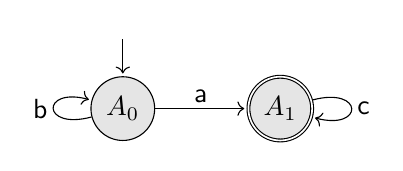
\begin{tikzpicture}[aut]
      \node[st,initial above]  (s_0) {$A_0$};
      \node[st,final] (s_1) [right of=s_0] {$A_1$};
      \path[->]
        (s_0) edge  node {a}  (s_1)
        (s_0) edge[loop left] node {b}  ()
        (s_1) edge[loop right] node {c}  (s_0);
    \end{tikzpicture}}
    ~~~~~~~~~~
    \wrap{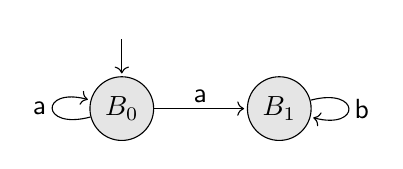
\begin{tikzpicture}[aut]
      \node[st,initial above]  (s_0) {$B_0$};
      \node[st] (s_1) [right of=s_0] {$B_1$};
      \path[->]
        (s_0) edge  node {a}  (s_1)
        (s_0) edge[loop left] node {a}  ()
        (s_1) edge[loop right] node {b}  (s_0);
    \end{tikzpicture}}
    \\[6mm]
    \wrap{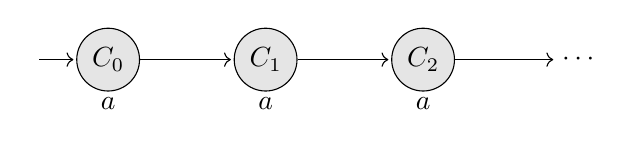
\begin{tikzpicture}[aut]
      \node[st,initial left]  (s_0) {$C_0$};
      \node[st] (s_1) [right of=s_0] {$C_1$};
      \node[st] (s_2) [right of=s_1] {$C_2$};
      \node (s_3) [right of=s_2] {$\cdots$};
      \node[below] at(s_0.south){$a$};
      \node[below] at(s_1.south){$a$};
      \node[below] at(s_2.south){$a$};
      \path[->]
        (s_0) edge (s_1)
        (s_1) edge  (s_2)
        (s_2) edge  (s_3);
    \end{tikzpicture}}
  }
\end{slide}


\begin{frame}{Our First encounter with Coalgebra}

  Indeed the idea of working at the level of

  \begin{center}
    \alert{Functors as Transition Types}
  \end{center}

  is a very fruitful one; and which we only barely
  grasped %(yet)
  ---

  in essence, it provides a \alert{universal theory} of transition
  systems that can be instantiated to most kinds of transition system
  we will encounter in our life
\end{frame}





\section{CCS Process algebra}

%-------------------------------------------------------------------------------
\begin{slide}{CCS Process algebra}
\small

\begin{block}{Sequential CCS - Syntax}
\begin{equation*}
% \mathcal{P} ~\ni~ P,Q\; ::=\; K ~~|~~ \alpha.P ~~|~~ \sum_{i\in I} P_i
%         ~~|~~ \crn P f \faded{~~|~~ P|Q ~~|~~ P\backslash L}
\mathcal{P} ~\ni~ P,Q\; ::=\; K ~~|~~ \alpha.P ~~|~~ P + Q ~~|~~ \cnil
        ~~|~~ \crn P f  ~~|~~ P\backslash L \faded{~~|~~ P|Q}
\end{equation*}
%
where
\\- $\alpha \in \Act %\faded{\cup \overline\Act \cup \set{\tau}}
    \cup \set{\tau}$~ is an \structure{action}
\\- $K$ s a collection of \structure{process} names or process constants
% \\- $I$ is an indexing set
\\- $L \subseteq \Act %\faded{\cup \overline{\Act}}
    $ is a set of \structure{labels}
\\- $f$ is a function that \structure{renames} actions s.t. $f(\tau) = \tau$ % and $f(\overline{a}) = \overline{f(a)}$
\\- \alert{notation:}
% \\~~~~~$\cnil = \sum_{i\in\emptyset}P_i$
% \\~~~~~$P_1+P_2 = \sum_{i\in\set{1,2}}P_i$
\\~~~~~$[f] = [a_1\mapsto b_1,\ldots,a_n \mapsto b_n]$
\end{block}
\end{slide}

%-------------------------------------------------------------------------------

\begin{slide}{CCS Process algebra}
\small

\begin{block}{Syntax}
\begin{equation*}
% \mathcal{P} ~\ni~ P,Q\; ::=\; K ~~|~~ \alpha.P ~~|~~ \sum_{i\in I} P_i
%         ~~|~~ \crn P f \faded{~~|~~ P|Q ~~|~~ P\backslash L}
\mathcal{P} ~\ni~ P,Q\; ::=\; K ~~|~~ \alpha.P ~~|~~ P + Q ~~|~~ \cnil
        ~~|~~ \crn P f  ~~|~~ P\backslash L \faded{~~|~~ P|Q}
\end{equation*}
\end{block}

%\setcounter{equation}{0}
\begin{exampleblock}{\exercise Which are NOT syntactically correct? Why?}
\begin{columns}
  \column{0.38\textwidth}
  \begin{align}
    & a.b.A+B\\&
    (a.\cnil + b.A) \backslash \set{a,b,c}\\&
    (a.\cnil + b.A) \backslash \set{a,\tau}\\& % no
    a.B+[b\mapsto a]\\& % no
    \tau.\tau.B + \cnil
  \end{align}

  \column{0.45\textwidth}
  \begin{align} &
    a.(a + b).A\\&
    (a.B + b.B)[a\mapsto a,\tau\mapsto b]\\&
    (a.B + \tau.B)[b\mapsto a,a\mapsto a]\\& % no
    % (a.b.A + \ainv a.\cnil)|B\\&
    (a.b.A + b.\cnil).B\\&
    (a.b.A + b.\cnil)+B
    % \\&
    % (\cnil | \cnil) + \cnil
  \end{align}
\end{columns}
\end{exampleblock}

\end{slide}

%-------------------------------------------------------------------------------

\exerciseBack
\begin{slide}{CCS semantics - building a transition system}
\small 
Every $P$ yields a transition system $X \to {\alert{???}}$ with transitions prescribed by the rules below.

\vspace*{-1mm}
\centering
\newcommand{\msep}{~~~~~~}

\typerule{act}{\shrk}{\alpha.P \trans\alpha P}
\msep
\typerule{sum-1}{P_1 \trans\alpha P'_1}{P_1 + P_2 \trans\alpha P'_1} %$\faded{j\in I}$
\msep
\typerule{sum-2}{P_2 \trans\alpha P'_2}{P_1 + P_2 \trans\alpha P'_2} %$\faded{j\in I}$
\\[3mm]
\typerule{res}{P\trans\alpha P'}{\crt P L\trans\alpha \crt{P'}L}~${\alpha%,\ainv{\alpha}
                                                                  \notin L}$
\msep
\typerule{rel}{P\trans\alpha P'}{\crn P f\trans{f(\alpha)} \crn{P'} f}
% \\[3mm]
% \typerule{com1}{P\trans\alpha P'}{P|Q\trans\alpha P'|Q}
% \msep
% \typerule{com2}{Q\trans\alpha Q'}{P|Q\trans\alpha P|Q'}
% \msep
% \typerule{com3}{P\trans a P' \quad Q\trans{\ainv{a}} Q'}{P|Q\trans\tau P'|Q'}
\\[6mm]

\only<1>{
  \begin{itemize}
    \item \structure{Initial states:} the process being translated
    \item \structure{Final states:} all states are final
    \item \alert{Language:} possible sequence of actions of a process
  \end{itemize}
}
\pause

\begin{exampleblock}{\exercise Build a derivation tree to prove the transitions below}
  \vspace*{-2mm}
  \begin{enumerate}
    \item $(a.A + b.B) ~\trans{b}~ B$
    \item $(a.b.A + (b.a.B + c.a.C)) ~\trans{b}~ a.B$
    \item $((a.B + b.A)[a \mapsto c])\backslash\{a,b\} ~\trans{c}~ (B[a\mapsto c])\backslash\{a,b\}$
  \end{enumerate}
\end{exampleblock}

\end{slide}

\begin{slide}{Exercise}
  \begin{exampleblock}{\exercise Draw the automata}
  % \vspace*{-4mm}
  \begin{align*}
    CM &= \mathsf{coin.coffee}.CM
    \\
    CS &= \mathsf{pub.(coin.coffee.CS + coin.tea.CS)}
    % CM &= \mathsf{coin.\ainv{coffee}}.CM
    % \\
    % CS &= \mathsf{\ainv{pub}.\ainv{coin}.coffee}.CS
    % \\
    % SmUni &= \crt{(CM|CS)}{\mathsf{\set{coin,coffee}}}
  \end{align*}
\end{exampleblock}

\doExercise{What is the language of the process $A$?}{
\centering
  \vspace*{-5mm}
  \begin{align*}
    A &= \mathsf{goLeft.A + goRight.B}
    \\
    B &= \mathsf{rest.\cnil}
  \end{align*}
}
\end{slide}


\begin{slide}{Exercise}
  \centering

  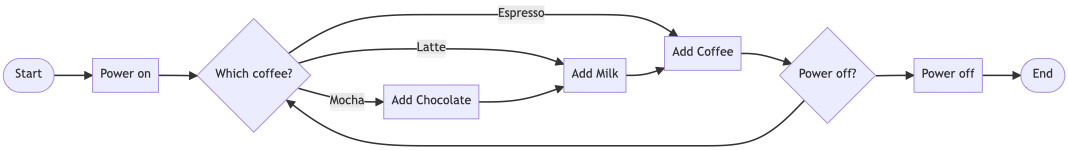
\includegraphics[width=1.0\textwidth]{images/coffee-flow.png}

  \doExercise{Write the process of the flowchart above}{
        $P ~~=~ \mf{powerOn} . Q$\\
        $Q ~~=~ \mf{selMocha}.\mf{addChocolate}.Mk + \mf{selLatte}.Mk + \ldots $\\
        $Mk ~=~ \mf{addMilk}\ldots$  
      ~\\[0.35\textheight]
  }

\end{slide}



% ----------------------------------------

\section{Concurrent Process algebra}


\begin{slide}{Overview}

\begin{block}{Recall}
\begin{enumerate}
  \item Non-deterministic Finite Automata ($X \to \faded{\mathtt{Bool}} \times \mathtt{P}(X)^{\Act}$):
  \wrap{\small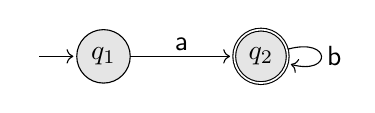
\begin{tikzpicture}[aut]
  \node[st,initial]  (q1) {$q_1$};
  \node[st,final] (q2) [right of=q1]  {$q_2$};
  \path[->] (q1) edge node {a} (q2) (q2) edge[loop right] node {b} ();
\end{tikzpicture}}
  \item (Sequential) Process algebra:
    $P = a.Q ~~~~ Q=b.Q$

  \item Meaning of \structure{(2)} using \structure{(1)}
\end{enumerate}  
\end{block}

\begin{block}{Still missing}
\begin{itemize}
  \item \alert{\textbf{Interaction}} between processes
  % \item \emph{Interaction \alert{diagrams}} vs. \emph{interacting \alert{processes}}
  \item Enrich \structure{(2)} and \structure{(3)}
\end{itemize}
\end{block}

\end{slide}

%-------------------------------------------------------------------------------
\begin{slide}{Process algebras}
\small

\begin{block}{CCS - \alert{Updated} Syntax}
\begin{equation*}
% \mathcal{P} ~\ni~ P,Q\; ::=\; K ~~|~~ \alpha.P ~~|~~ \sum_{i\in I} P_i
%         ~~|~~ \crn P f \transp{~~|~~ P|Q ~~|~~ P\backslash L}
\mathcal{P} ~\ni~ P,Q\; ::=\; K ~~|~~ \alpha.P ~~|~~ P + Q ~~|~~ \cnil
        ~~|~~ \crn P f  ~~|~~ P\backslash L ~~|~~ \alert{P|Q}
\end{equation*}
%
where
\\- $\alpha \in \Act \alert{\cup \overline\Act}
    \cup \set{\tau}$~ is an action
\\- $K$ s a collection of process names or process constants
\\- $L \subseteq \Act %\transp{\cup \overline{\Act}}
    $ is a set of labels
\\- $f$ is a function that renames actions s.t. $f(\tau) = \tau$  \alert{and $f(\overline{a}) = \overline{f(a)}$}
\\- notation:
% \\~~~~~$\cnil = \sum_{i\in\emptyset}P_i$
% \\~~~~~$P_1+P_2 = \sum_{i\in\set{1,2}}P_i$
\\~~~~~$[f] = [a_1\mapsto b_1,\ldots,a_n \mapsto b_n]$~~~~~where \alert{$a_i,b_i \in N \cup \set{\tau}$}
\end{block}
\end{slide}

%-------------------------------------------------------------------------------

\begin{slide}{Process algebras}
\small

\begin{block}{Syntax}
\begin{equation*}
% \mathcal{P} ~\ni~ P,Q\; ::=\; K ~~|~~ \alpha.P ~~|~~ \sum_{i\in I} P_i
%         ~~|~~ \crn P f \transp{~~|~~ P|Q ~~|~~ P\backslash L}
\mathcal{P} ~\ni~ P,Q\; ::=\; K ~~|~~ \alpha.P ~~|~~ P + Q ~~|~~ \cnil
        ~~|~~ \crn P f  ~~|~~ P\backslash L ~~|~~  \alert{P|Q}
\end{equation*}
\end{block}

%\setcounter{equation}{0}
\begin{exampleblock}{\exercise Which are syntactically correct?}
\begin{columns}
  \column{0.38\textwidth}
  \begin{align}
    & a.\ainv b.A+B\\&
    (a.\cnil + \ainv a.A) \backslash \set{\ainv{a},b}\\&
    (a.\cnil + \ainv a.A) \backslash \set{a,\tau}\\& % no
    (a.\cnil + \ainv{\tau}.A) \backslash \set{a}\\& % no
    % a.B+[b\mapsto a]\\& % no
    \tau.\tau.B + \ainv a.\cnil %\\&
    % a.(a + b).A
    \\&
    (\cnil | \cnil) + \cnil
  \end{align}

  \column{0.45\textwidth}
  \begin{align} &
    (a.B + b.B)[a\mapsto a,\tau\mapsto b]\\&
    (a.B + \tau.B)[b\mapsto a,b\mapsto a]\\& % no
    (a.B + b.B)[a\mapsto b,b\mapsto \ainv a]\\& % no
    (a.b.A + \ainv a.\cnil)|B\\&
    (a.b.A + \ainv a.\cnil).B\\&
    (a.b.A + \ainv a.\cnil)+B
  \end{align}
\end{columns}
\end{exampleblock}

\end{slide}

%-------------------------------------------------------------------------------

\begin{slide}{CCS semantics - building an NFA}
\small 
\centering
\newcommand{\msep}{~~~~~~}
\vspace*{-2mm}

\typerule{act}{\shrk}{\alpha.P \trans\alpha P}
\msep
\typerule{sum-1}{P_1 \trans\alpha P'_1}{P_1 + P_2 \trans\alpha P'_1} %$\transp{j\in I}$
\msep
\typerule{sum-2}{P_2 \trans\alpha P'_2}{P_1 + P_2 \trans\alpha P'_2} %$\transp{j\in I}$
\\[2mm]
\typerule{res}{P\trans\alpha P'}{\crt P L\trans\alpha \crt{P'}L}~$\transp{\alpha,\ainv{\alpha}
                                                                  \notin L}$
\msep
\typerule{rel}{P\trans\alpha P'}{\crn P f\trans{f(\alpha)} \crn{P'} f}
\\[2mm]
\alert{
\typerule{com1}{P\trans\alpha P'}{P|Q\trans\alpha P'|Q}
\msep
\typerule{com2}{Q\trans\alpha Q'}{P|Q\trans\alpha P|Q'}
\msep
\typerule{com3}{P\trans a P' \quad Q\trans{\ainv{a}} Q'}{P|Q\trans\tau P'|Q'}
}
\\[2mm]
\pause

\begin{exampleblock}{\exercise Draw the transition systems}
  \exerciseBack
  \vspace*{-5mm}
  \begin{align*}
    % CM &= \mathsf{coin.coffee}.CM
    % \\
    % CS &= \mathsf{pub.(coin.coffee.CS + coin.tea.CS)}
    CM &= \mathsf{coin.\ainv{coffee}}.CM
    \\
    CS &= \mathsf{pub.\ainv{coin}.coffee}.CS
    \\
    SmUni &= \crt{(CM|CS)}{\mathsf{\set{coin,coffee}}}
  \end{align*}
  \vspace*{-7mm}
\end{exampleblock}
\end{slide}
\exerciseAdd



\begin{slide}{Exercises}
  \doExercise{Let $A=b.a.B$. Show that:}{
    \vspace*{-8mm}
    \begin{enumerate}
      \item $(A ~|~ \overline{b}.\cnil)\backslash \{b\}~\trans\tau~ (a.B ~|~ \cnil)\backslash\{b\}$
      \item $(A ~|~ b.a.B) + ((b.A)[b\mapsto a]) ~\trans{a}~ A[b \mapsto a]$
    \end{enumerate}
  }  

  \doExercise{Draw the NFAs $A$ and $D$}{
    \vspace*{-8mm}

    \begin{columns}
    \col[0.45]{      
    \begin{align*}
      A &= x.B+x.x.C\\
      B &= x.x.A+y.C\\
      C &= x.A      
    \end{align*}
    }
    \col[0.45]{      
    \begin{align*}
      D &= x.x.x.D + x.E\\
      E &= x.F+y.F\\
      F &= x.D      
    \end{align*}
    }
    \end{columns}
  }  

\end{slide}


\begin{frame}
  \huge\centering
  mCRL2 Tools  -- generate automata
  \\[5mm]\large
  Slides 3:\\\url{https://fm-dcc.github.io/sv2425/slides/3-mcrl2.pdf}
\end{frame}



\section{Observational Equivalence}

\begin{slide}{Overview}

\begin{block}{Recall}
\begin{enumerate}
  \item F-transition systems, e.g., Non-deterministic Finite Automata:
  \wrap{\small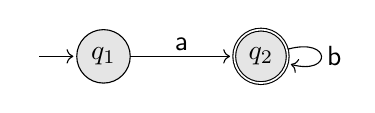
\begin{tikzpicture}[aut]
  \node[st,initial]  (q1) {$q_1$};
  \node[st,final] (q2) [right of=q1]  {$q_2$};
  \path[->] (q1) edge node {a} (q2) (q2) edge[loop right] node {b} ();
\end{tikzpicture}}
  \item Process algebra:
    $P = a.Q ~~~~ Q=b.Q ~~~~ P|Q$

  \item Interaction between processes
  
  \item Meaning of CCS using transition systems

  % \item Equivalence relations ((bi)simulations)
\end{enumerate}  
\end{block}

\begin{block}{Still missing}
\begin{itemize}
  \item When is a process $P$ \alert{equivalent} to a process $Q$?
  \item When can a process $P$ be \alert{safely replaced} by a process $Q$?
  % \item When can a sequence of interactions be \alert{safely implemented} as interacting components?
\end{itemize}
\end{block}
\end{slide}


\begin{frame}{Observational Equivalence Informally}

  Two programs are \structure{observationally equivalent} if it is impossible to \alert{observe any
  difference} in their \alert{behaviour}

  
  \vfill
  Here behaviour is described in terms of transition systems

  \dots\ and therefore behaviour/equivalence needs to be pinned
  down to them
\end{frame}

\section{EQ1 -- Language equivalence}

%----------------------------------------------------------------------------------
\begin{slide}{Language  equivalence}
\small

\begin{block}{Definition}
Two automata $A, B$ are \alert{language equivalent} iff  $ L_A =  L_B$\\
(i.e. if they can perform the same finite sequences of transitions)
\end{block}
~\\

\begin{example}
  \centering
  % Requires \usepackage{graphicx}
  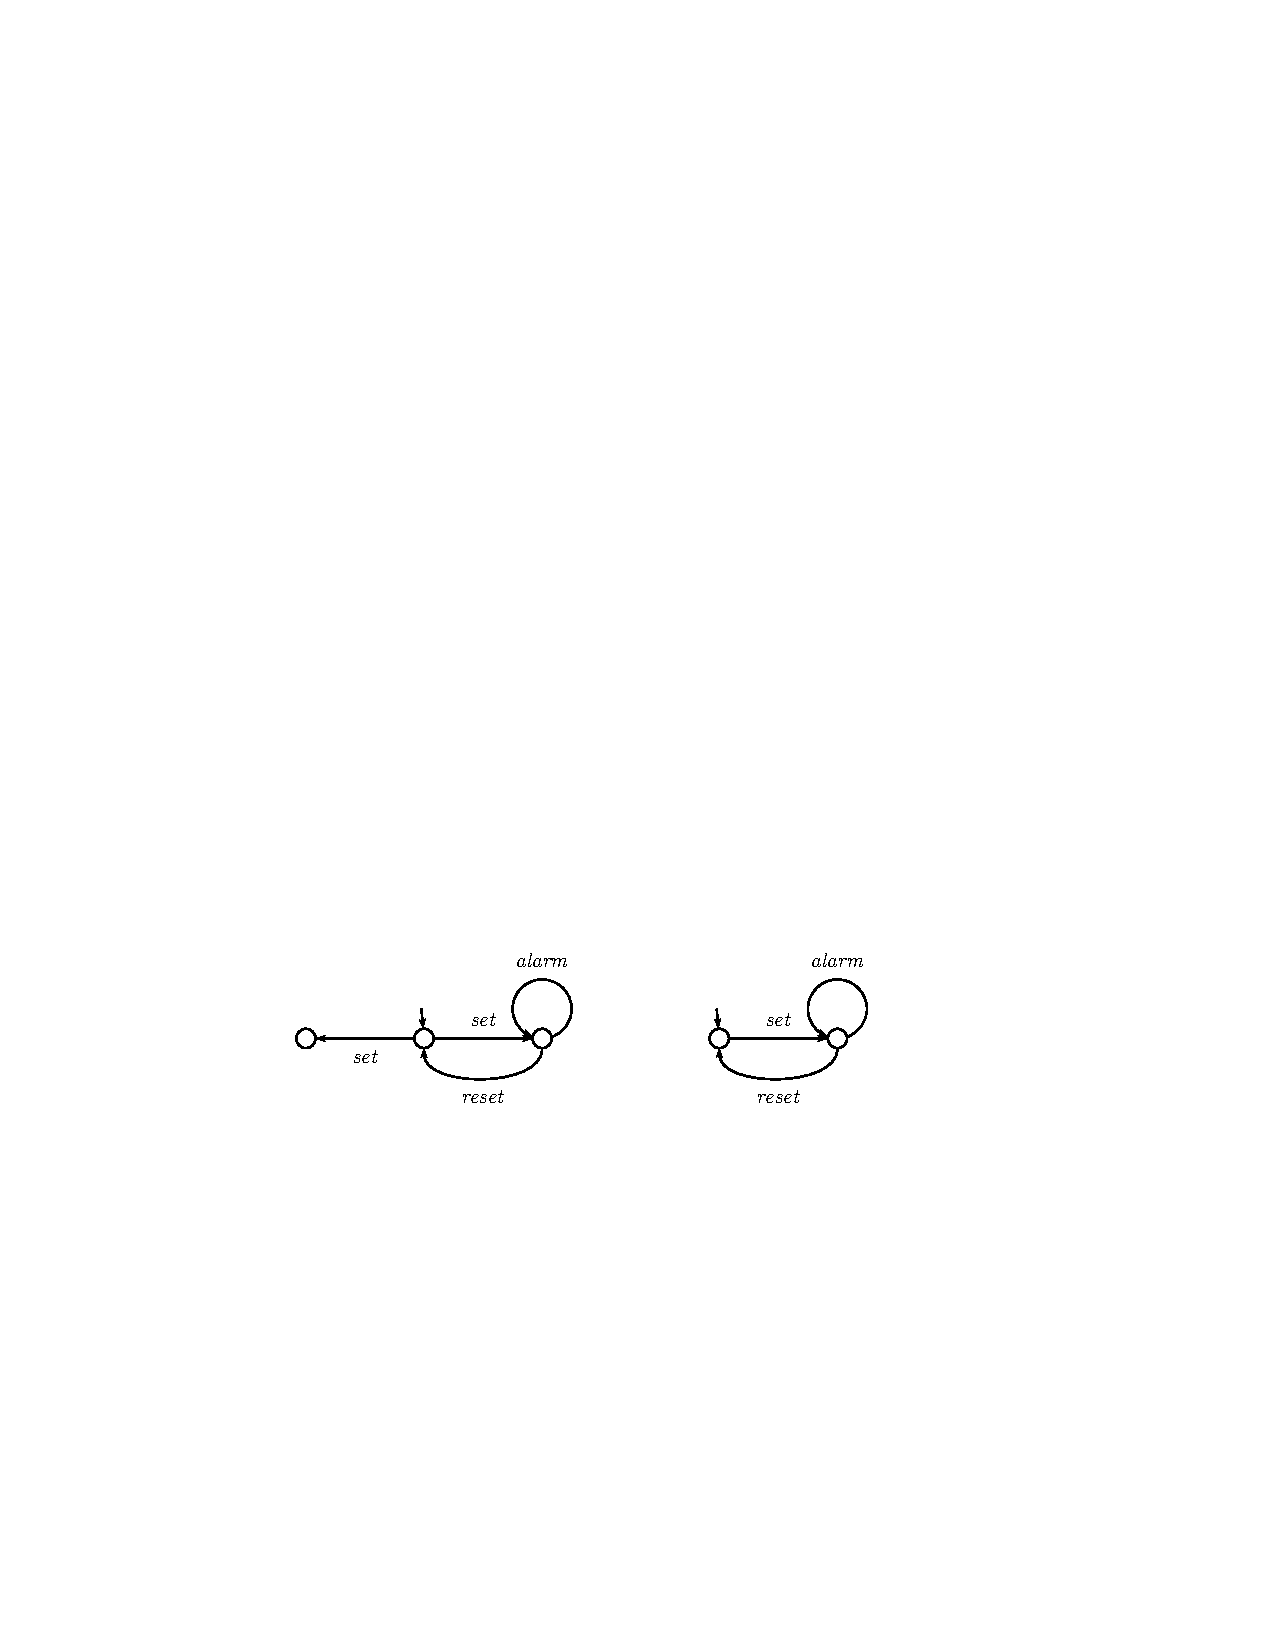
\includegraphics[width=9cm]{./images/alarm3.pdf}
\end{example}


\alert{Language equivalence} applies  when one can neither interact with a system, nor distinguish a slow system from one that has come to a stand still.
\end{slide}


% \begin{slide}{Exercise}
%   \centering
%   \doExercise{Consider the system}{
%   \centering
%   \begin{tikzpicture}
%       \node(p){$p$}; \node[right=of p](p1){$p_1$}; \node[right=of p1](p2){$p_2$};
%       \draw[->] (p)edge[bend right] node[below]{a} (p1)
%                 (p1)edge[bend right] node[above]{b}(p)
%                 (p2)edge node[above]{d} (p1)edge[loop right] node[right]{c}(p1) ;
%   \end{tikzpicture}
%   \begin{enumerate}
%     \item Formalise the system as a tuple $(S,Act,\to)$
%     \item List 4 different traces from state (p2).
%   \end{enumerate}
%   }
% \end{slide}


\begin{slide}{Exercise}
  \centering
  \doExercise{Find pairs of automata with the same language}{
    \centering 
    \wrap{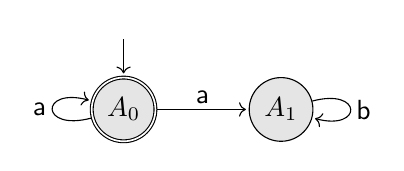
\begin{tikzpicture}[aut]
      \node[st,initial above,final]  (s_0) {$A_0$};
      \node[st] (s_1) [right of=s_0] {$A_1$};
      \path[->]
        (s_0) edge  node {a}  (s_1)
        (s_0) edge[loop left] node {a}  ()
        (s_1) edge[loop right] node {b}  (s_0);
    \end{tikzpicture}}
    ~~~~~~~~~~
    \wrap{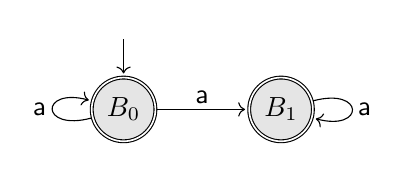
\begin{tikzpicture}[aut]
      \node[st,initial above,final]  (s_0) {$B_0$};
      \node[st,final] (s_1) [right of=s_0] {$B_1$};
      \path[->]
        (s_0) edge  node {a}  (s_1)
        (s_0) edge[loop left] node {a}  ()
        (s_1) edge[loop right] node {a}  (s_0);
    \end{tikzpicture}}
    ~~~~~~~~~
    \wrap{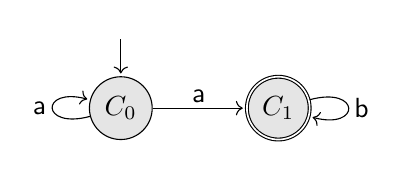
\begin{tikzpicture}[aut]
      \node[st,initial above]  (s_0) {$C_0$};
      \node[st,final] (s_1) [right of=s_0] {$C_1$};
      \path[->]
        (s_0) edge  node {a}  (s_1)
        (s_0) edge[loop left] node {a}  ()
        (s_1) edge[loop right] node {b}  (s_0);
    \end{tikzpicture}}
    ~~~~~~~~~
    \wrap{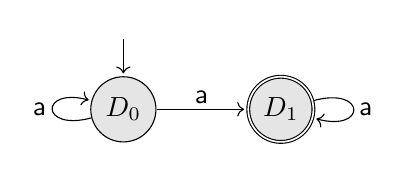
\begin{tikzpicture}[aut]
      \node[st,initial above]  (s_0) {$D_0$};
      \node[st,final] (s_1) [right of=s_0] {$D_1$};
      \path[->]
        (s_0) edge  node {a}  (s_1)
        (s_0) edge[loop left] node {a}  ()
        (s_1) edge[loop right] node {a}  (s_0);
    \end{tikzpicture}}
    ~~~~~~~~~
    \wrap{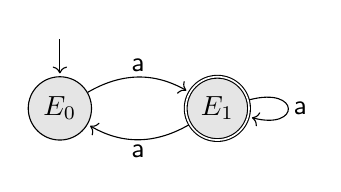
\begin{tikzpicture}[aut]
      \node[st,initial above]  (s_0) {$E_0$};
      \node[st,final] (s_1) [right of=s_0] {$E_1$};
      \path[->]
        (s_0) edge[bend left]  node {a}  (s_1)
        (s_1) edge[bend left]  node {a}  (s_0)
        (s_1) edge[loop right] node {a}  (s_0);
    \end{tikzpicture}}

  }
\end{slide}

\begin{slide}{Exercise}
  \doExercise{Check if the processes are language equivalent}{
    \begin{align*}
      P &= coin.(\ainv{coffee}.P + \ainv{tea}.P)
      &
      Q &= coin.\ainv{coffee}.Q + coin.\ainv{tea}.Q
    \end{align*}
  }

\end{slide}


\section{EQ2 -- Similarity}

%----------------------------------------------------------------------------------
\begin{slide}{Simulation}
\begin{flushright}
the quest for a \alert{behavioural equality}:\\
able to identify states that cannot be distinguished by any \alert{realistic} form of  observation
\end{flushright}
~\\

\small
\begin{block}{Simulation}
% \caixa
{A state $q$ \alert{simulates} another state $p$
\alert{if}\\
every transition from $q$ is corresponded by a transition from $p$
\alert{and}\\
this capacity is kept along the whole life of the system to which state space $q$ belongs to.}
\end{block}
\end{slide}

%----------------------------------------------------------------------------------
\begin{slide}{Simulation of NFA ($X \to \mathtt{P}(X)^{\Act}$)}
\small

\begin{block}{Definition}
% Given  $\pair{S_1, \Act, \rra_1}$  and $\pair{S_2, \Act, \rra_2}$
%  over $\Act$ \faded{(ignoring initial and final states)}
Given NFA $A_1$ and $A_2$ over \Act\ with states $S_1$ and $S_2$ respectively,
a relation \structure{$R \subseteq S_1 \times S_2$} is a \structure{simulation} iff,
for all $\pair{p,q} \in \structure{R}$ and $a \in \Act$,

\begin{align*}
%\text{\gold{(1)}}\; \;  & p \downarrow_1 \;  \imp\; q \downarrow_2\\ &\\
\text{\alert{(1)}}\; \;  & p \rtran{a}_1 p'\;  \imp\; \rcb{\exists}{q'}{q' \in S_2}{q \rtran{a}_2 q'\, \land\, \pair{p',q'} \in \structure{R}}   
\end{align*}
\vspace{0mm}

\begin{equation*}
\xymatrix{
p \ar[d]^-{a} & \hspace{-1.5cm} \structure{R}  & \hspace{-2.7cm} q 
  & \!\! \text{\raisebox{-10mm}{\Huge $\imp$}} \! \! &  &  &  q \ar[d]^-{a} \\
p'           &   &           &                                   & p'\hspace{-2.7cm} &  \structure{R} \hspace{-1.5cm} &  q'
}
\end{equation*}

\end{block}
\end{slide}

%----------------------------------------------------------------------------------
\begin{slide}{Example}

\begin{exampleblock}{\exercise Find simulations}
\begin{equation*}
\xymatrix{
& q_1  \ar[r]^{d} & q_2 &       &        &                              p_2\\
q_0 \ar[ru]^{a} \ar[rd]_{a} &  & & p_0 \ar[r]^{a} & p_1 \ar[ru]^{d} \ar[rd]_{e} & \\
& q_4  \ar[r]_{e} & q_3 &       &        &                              p_3\\
}
\end{equation*}
\end{exampleblock}

\vspace{0.2cm}
\visible<2->{\exerciseBack\begin{equation*}
q_0 \lesssim p_0 \text{\hspace{0.5cm} cf. \hspace{0.3cm}} 
\set{\pair{q_0,p_0}, \pair{q_1,p_1},\pair{q_4,p_1},\alert{\ldots}} %\pair{q_2,p_2},\pair{q_3,p_3}}
\end{equation*}}
\end{slide}

\exerciseAdd


%----------------------------------------------------------------------------------
\begin{slide}{Similarity}
\small

\begin{block}{Definition}
\centering
\[p \lesssim q\; \equiv\; \rcb{\exists}{R}{}{R\; \text{is a simulation and}\; \pair{p,q} \in R} 
\]
\emph{We say \alert{$p$ is simulated by $q$}.}
\end{block}

% \begin{block}{Automata simulation}
%   \[\pair{S_1,\set{s_1},\dda_1,\rra_1} \lesssim \pair{S_2,\set{s_2},\dda_2,\rra_2}\; \equiv\; s_1 \lesssim s_2 
% \]
% \end{block}

\begin{block}{Lemma}
The similarity relation is a preorder\\
\faded{(ie, reflexive and transitive)}
\end{block}
\end{slide}



%-------------------------

\section{EQ3 -- Bisimilarity}
%----------------------------------------------------------------------------------
\begin{slide}{Bisimulation}
\small

\begin{block}{Definition}
% Given  $\pair{S_1, \Act,  \rra_1}$  and $\pair{S_2, \Act, \rra_2}$ over $\Act$,
Given NFA $A_1$ and $A_2$ over \Act\ with states $S_1$ and $S_2$ respectively,
relation $R \subseteq S_1 \times S_2$ is a \structure{bisimulation} iff both $R$ and its converse $\aconv{R}$
are simulations.

I.e.,
whenever $\pair{p,q} \in R$ and $a \in \Act$,

\begin{align*}
%\text{\gold{(1)}}\; \;  &  p \downarrow_1 \;  \dimp\; q \downarrow_2\\ &\\
\text{\alert{(1)}}\; \;  & p \rtran{a}_1 p'\; \imp\; \rcb{\exists}{q'}{q' \in S_2}{q \rtran{a}_2 q'\, \land\, \pair{p',q'} \in R}   \\
\text{\alert{(2)}}\; \;  & q \rtran{a}_2 q'\; \imp\; \rcb{\exists}{p'}{p' \in S_1}{p \rtran{a}_1 p'\, \land\, \pair{p',q'} \in R}   
\end{align*}

%\begin{equation*}
%\xymatrix{
%p \ar[d]^-{a} & \hspace{-1.5cm} R  & \hspace{-2.7cm} q
%    & \! \! \text{\raisebox{-10mm}{\Huge $\Leftrightarrow$}} \! \! &   &  
%    &  q \ar[d]^-{a} \\
%p'           &   &           &                                   & p'\hspace{-2.7cm} &  R \hspace{-1.5cm} &  q'
%}
%\end{equation*}
\centering
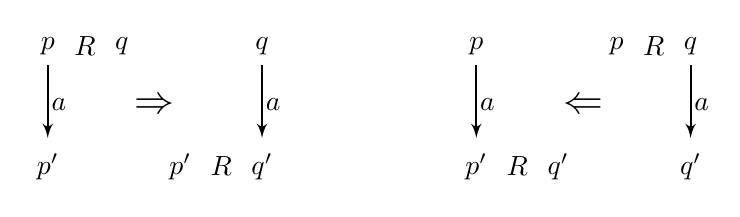
\begin{tikzpicture}[%
    every edge/.style={draw, thick,-latex',shorten >= 2pt}]
  \tikzstyle{l} = [auto,inner sep=1pt]
  % the square
  \node(p){$p$};\node[right=2.3 of p](q2){$q$};
  \node[below=1 of p](p'){$p'$};\node(q')at(p'-|q2){$q'$};
  % the R parts
  \node[right=0 of p](R1){$R$};\node[right=0 of R1](q){$q$};
  \node[left=0 of q'](R2){$R$};\node[left=0 of R2](p'2){$p'$};
  % the arrows
  \draw[->] (p)edge node[l]{$a$}(p') (q2)edge node[l]{$a$}(q');
  \node at ($(p)!.5!(q')$){{\Large $\Rightarrow$}};
  %%%%%%%
  % the square
  \node[right=2.3 of q2](pp){$p$};\node[right=2.3 of pp](q2){$q$};
  \node[below=1 of pp](p'){$p'$};\node(q')at(p'-|q2){$q'$};
  % the R parts
  \node[right=0 of p'](R1){$R$};\node[right=0 of R1](q){$q'$};
  \node[left=0 of q2](R2){$R$};\node[left=0 of R2](p'2){$p$};
  % the arrows
  \draw[->] (pp)edge node[l]{$a$}(p') (q2)edge node[l]{$a$}(q');
  \node at ($(pp)!.5!(q')$){{\Large $\Leftarrow$}};

\end{tikzpicture}

\end{block}
\end{slide}



%----------------------------------------------------------------------------------
\begin{slide}{Examples}

\doExercise{Find bisimulations that include $\pair{q_1,m}$}{
\begin{equation*}
\xymatrix{
& q_1  \ar[ld]_{a}  \ar[rd]^{a} & & & & m \ar[d]_{a}\\
q_2 \ar[rr]^{c}  && q_3 \ar@(ur,dr)[]^{c}  & & & n\ar@(ur,dr)[]^{c}
}
\end{equation*}
% R = \enset{(q_1,m), (q_2, n), (q_3,n) }
}

\doExercise{Find bisimulations that include $\pair{q_1,h}$}{

\begin{equation*}
\xymatrix{
q_1 \ar[r]^{a} & q_2  \ar[r]^{a}  & q_3  \ar[r]^{a} & \cdots & & h\ar@(ur,dr)[]^{a}  \\
}
\end{equation*}
% R = \setdef{q_i, h}{i \geq 1}  
}

\end{slide}



% Definition
% p∼q ≡ ⟨∃R :: Risabisimulationand⟨p,q⟩∈R⟩
%----------------------------------------------------------------------------------
\begin{slide}{Bisimilarity}
\small

\begin{block}{Definition}
\centering
\[p \sim q\; \equiv\; \rcb{\exists}{R}{}{R\; \text{is a bisimulation and}\; \pair{p,q} \in R} 
\]
\emph{We say \alert{$p$ is bisimilar to $q$}.}
\end{block}


\begin{block}{Lemma}
\centering
Two processes $P$ and $Q$ are bisimilar if there is a bisimulation that includes $\pair{P,Q}$.
\end{block}

\begin{block}{Lemma}
The bisimilarity relation is an equivalence relation\\
\faded{(ie, symmetric, reflexive and transitive)}
\end{block}


% \begin{block}{Automata simulation}
%   \[\pair{S_1,\set{s_1},\dda_1,\rra_1} \lesssim \pair{S_2,\set{s_2},\dda_2,\rra_2}\; \equiv\; s_1 \lesssim s_2 
% \]
% \end{block}

% \begin{block}{Lemma}
% The similarity relation is a preorder\\
% \faded{(ie, reflexive and transitive)}
% \end{block}
\end{slide}



%----------------------------------------------------------------------------------
\begin{slide}{Exercises}

\doExercise{Check if there is a bisimulation that include $\pair{q_1,p_1}$}{
\vspace*{-3mm}
\begin{equation*}
\xymatrix{
& q_1  \ar[ld]_{a}  \ar[rd]^{a} & & & & p_1  \ar[d]^{a} \\
q_2 \ar[d]^{c}  && q_3  \ar[d]^{c}  & && p_2  \ar[ld]_{c}  \ar[rd]^{c} & \\
q_4 & & q_5 & &p_4 & & p_5\\
% & q_1  \ar[ld]_{a}  \ar[rd]^{a} & & & & p_1  \ar[d]^{a} \\
% q_2 \ar[d]^{\rdb{b}}  && q_3  \ar[d]^{c}  & && p_2  \ar[ld]_{\rdb{b}}  \ar[rd]^{c} & \\
% q_4 & & q_5 & &p_4 & & p_5
}
\end{equation*}
}

\doExercise{Check if there is a bisimulation that include $\pair{P,Q}$}{
  \vspace*{-5mm}
  \begin{align*}
      P &= coin.(\ainv{coffee}.P + \ainv{tea}.P)
      &
      Q &= coin.\ainv{coffee}.Q + coin.\ainv{tea}.Q
  \end{align*}
}
\end{slide}


\begin{slide}{Exercises}
\doExercise{Check if there is a bisimulation that include $\pair{q_1,p_1}$}{
\vspace*{-3mm}
\begin{equation*}
\xymatrix{
% & q_1  \ar[ld]_{a}  \ar[rd]^{a} & & & & p_1  \ar[d]^{a} \\
% q_2 \ar[d]^{c}  && q_3  \ar[d]^{c}  & && p_2  \ar[ld]_{c}  \ar[rd]^{c} & \\
% q_4 & & q_5 & &p_4 & & p_5\\
& q_1  \ar[ld]_{a}  \ar[rd]^{a} & & & & p_1  \ar[d]^{a} \\
q_2 \ar[d]^{\rdb{b}}  && q_3  \ar[d]^{c}  & && p_2  \ar[ld]_{\rdb{b}}  \ar[rd]^{c} & \\
q_4 & & q_5 & &p_4 & & p_5
}  
\end{equation*}
}

\doExercise{Check if, for any process P}{
  \vspace*{-5mm}
  \begin{align*}
      P ~\sim~ P + \cnil
  \end{align*}
}

\end{slide}


\begin{frame}
  \huge\centering
  mCRL2 Tools -- check bisimilarity
  \\[5mm]\large
  Slides 3:\\\url{https://fm-dcc.github.io/sv2425/slides/3-mcrl2.pdf}
\end{frame}





\section{Generalising Observational Equivalences}

\begin{frame}{$F$-Transition Systems and Observational \underline{Equivalence}}

  \begin{definition}
    Fix a functor $F$ and consider two transition systems
    $f : X \to F X$ and $g : Y \to F Y$. Two states $x \in X$, $y \in Y$
    are \alert{observationally equivalent if}
      \begin{itemize}
         \item there exists \structure{a relation}
      $\structure{R} \subseteq X \times Y$ with $(x,y) \in R$ and
         \item there exists \structure{a transition system} $\structure{b} : R \to FR$ such that the diagram below commutes
       \end{itemize} 
    \[
      \xymatrix{
        X \ar[d]_{f} & \ar[l]_{\pi_1}  \structure{R} \ar[r]^{\pi_2} \ar[d]_{\structure{b}} & Y \ar[d]^{g} \\
        F X  & \ar[l]^{F \pi_1} \structure{FR} \ar[r]_{F \pi_2} & F Y
        }
    \]
    If such is the case we write \alert{$x \sim y$}  
  \end{definition}
\end{frame}

\begin{frame}{Observational Equivalence for Moore Machine}
  Given $\pv{o_1}{n_1} : X \to A \times X$ and
  $\pv{o_2}{n_2} : Y \to A \times Y$ we obtain from the previous slide 
  that $x \sim y$ iff
  \begin{itemize}
  \item $o_1(x) = o_2(y)$
  \item $n_1(x) \sim n_2(y)$
  \end{itemize}
\end{frame}

\begin{frame}{Observational Equivalence for Labelled Transition Systems}
  Recall that we used systems of type $X \to \Pow(X)^\Act$ for establishing the
  \alert{semantics} of \alert{CCS processes}. This means that \dots

  notions of observational behaviour/equivalence for such transition systems
  directly impact our concurrent language

  \vfill Given $\overline{t_1} : X \to \Pow(X)^\Act$ and
  $\overline{t_2} : Y \to \Pow(Y)^\Act$, $x \sim y$ iff for all $l \in \Act$
  \begin{itemize}
  \item $\forall x' \in t_1(x,n).\  \exists y' \in t_2(y,n).\ x' \sim y'$
  \item $\forall y' \in t_2(y,n).\ \exists x' \in t_1(x,n).\ x' \sim y'$
  \end{itemize}
\end{frame}


% \begin{frame}{Is Observational Equivalence a Good Notion of Equivalence?}

%   \begin{block}{Coinduction Principle}
%       Two states $x,y$ are observationally \alert{equivalent} iff they produce the
%       \alert{same} observational behaviour
%   \end{block}
  
% \end{frame}

\end{document}
